% !TeX program = pdflatex
% Reconstrucao vetorial e tipografica do material "Quanto tempo podemos ficar no ar?"
% Equacoes, tabelas e graficos sao elementos LaTeX/TikZ/PGFPlots.
% As ilustracoes sao recortes transparentes extraidos das paginas originais, nunca slides completos.
\documentclass[aspectratio=169,11pt,professionalfonts]{beamer}
\usepackage[utf8]{inputenc}
\usepackage[T1]{fontenc}
\usepackage[brazil]{babel}
\usepackage{lmodern}
\usepackage{amsmath,amssymb,mathtools}
\usepackage{tikz}
\usetikzlibrary{arrows.meta,calc,positioning,decorations.pathreplacing,shapes.geometric}
\usepackage{pgfplots}
\pgfplotsset{compat=1.18}
\usepackage{booktabs,tabularx,array}
\usepackage{microtype}
\usepackage{hyperref}
\usepackage{graphicx}
\graphicspath{{ilustracoes_salto/}}

\definecolor{primary}{HTML}{173FA9}
\definecolor{accent}{HTML}{CB2734}
\definecolor{ink}{HTML}{18243B}
\definecolor{muted}{HTML}{586474}
\definecolor{paperbg}{HTML}{FBFAF7}
\definecolor{lightblue}{HTML}{E9F1FC}
\definecolor{softred}{HTML}{FFF1EE}
\definecolor{gridgray}{HTML}{CFD5DF}
\definecolor{basket}{HTML}{D97E2B}
\setbeamercolor{background canvas}{bg=paperbg}
\setbeamercolor{normal text}{fg=ink}
\setbeamercolor{frametitle}{fg=primary}
\setbeamercolor{structure}{fg=primary}
\setbeamerfont{frametitle}{size=\LARGE,series=\bfseries}
\setbeamerfont{footline}{size=\tiny}
\setbeamertemplate{navigation symbols}{}
\setbeamertemplate{itemize item}{\color{primary}\raisebox{0.20ex}{\scriptsize$\bullet$}}
\setbeamertemplate{itemize subitem}{\color{primary}\scriptsize$\circ$}
\setbeamersize{text margin left=0.82cm,text margin right=0.82cm}
\setbeamertemplate{frametitle}{%
  \vspace{0.17cm}%
  \begin{beamercolorbox}[wd=\paperwidth,leftskip=.82cm,rightskip=.82cm]{frametitle}%
    \usebeamerfont{frametitle}\insertframetitle\par\vspace{.06cm}%
    {\color{primary}\rule{14.36cm}{0.65pt}}%
  \end{beamercolorbox}%
}
\setbeamertemplate{footline}{%
 \leavevmode\hbox{%
 \begin{beamercolorbox}[wd=\paperwidth,ht=.38cm,dp=.12cm,leftskip=.82cm,rightskip=.82cm]{normal text}%
   {\color{gridgray}\rule{14.36cm}{.35pt}}\par\vspace{.025cm}%
   \color{muted}\scriptsize O. L. Santos-Pereira \hfill Cinemática vertical e hang time \hfill \insertframenumber\,/\,\inserttotalframenumber
 \end{beamercolorbox}}%
}
\newcommand{\eqcard}[1]{\tikz[baseline=(e.base)]{\node[draw=accent,rounded corners=2pt,line width=.9pt,fill=white,inner xsep=10pt,inner ysep=9pt] (e) {$\displaystyle #1$};}}
\newcommand{\bluecard}[1]{\tikz[baseline=(e.base)]{\node[draw=primary!55,rounded corners=2pt,line width=.7pt,fill=lightblue,inner xsep=10pt,inner ysep=7pt] (e) {#1};}}
\newcommand{\keyterm}[1]{\textcolor{primary}{\bfseries #1}}
\newcommand{\alertterm}[1]{\textcolor{accent}{\bfseries #1}}
\newcommand{\reftext}[1]{{\color{muted}\footnotesize #1}}
\newcommand{\sectionline}[1]{\vspace{.1cm}{\color{primary}\bfseries #1}\par\vspace{.07cm}}
\newcommand{\ball}[1][.19]{%
  \draw[fill=basket,draw=ink,line width=.6pt] (0,0) circle (#1);
  \draw[ink,line width=.5pt] (-#1,0)--(#1,0);
  \draw[ink,line width=.5pt] (0,-#1)--(0,#1);
  \draw[ink,line width=.5pt] (0,0) ellipse ({#1*.50} and #1);
}
\tikzset{
 pics/jumper/.style={code={
  \draw[line width=1.8pt,draw=ink] (0,1.54) circle (.14);
  \draw[line width=3.4pt,draw=primary] (0,1.37) -- (-.10,.70);
  \draw[line width=2pt,draw=ink] (-.10,.72)--(-.35,.27)--(-.48,.08);
  \draw[line width=2pt,draw=ink] (-.10,.72)--(.18,.33)--(.30,.18);
  \draw[line width=2pt,draw=ink] (-.07,1.26)--(.19,1.61)--(.25,1.95);
  \draw[line width=2pt,draw=ink] (.03,1.26)--(.34,1.56)--(.43,1.89);
  \draw[line width=2.3pt,draw=accent] (-.55,.08)--(-.40,.08);
  \draw[line width=2.3pt,draw=accent] (.30,.18)--(.43,.18);
 }},
 pics/hoop/.style={code={
  \draw[line width=1.3pt,draw=ink] (.6,1.65) -- (1.43,1.65)--(1.43,2.83)--(.6,2.83)--cycle;
  \draw[line width=.8pt,draw=gridgray] (.75,1.85) rectangle (1.26,2.48);
  \draw[line width=2pt,draw=accent] (.23,1.73) ellipse (.42 and .105);
  \foreach \x in {-0.11,0,0.11,0.22,0.33,0.44,0.55} {
     \draw[line width=.45pt,draw=muted] (\x,1.68)--({.23+(\x-.23)*.62},1.16);
  }
  \draw[line width=.55pt,draw=muted] (.00,1.45)--(.46,1.45);
  \draw[line width=.55pt,draw=muted] (.07,1.27)--(.39,1.27);
 }}
}
\title{Quanto tempo podemos ficar no ar?}
\subtitle{Uma introdução à cinemática vertical através do basquete}
\author{Osvaldo L. Santos-Pereira}
\institute{Instituto de Física\\Universidade Federal do Rio de Janeiro (UFRJ)}
\date{}
\begin{document}

% 01 --- CAPA

\begin{frame}[plain]
\begin{columns}[T,totalwidth=\textwidth]
\begin{column}{.53\textwidth}
\vspace{1.35cm}
{\fontsize{29}{35}\selectfont\bfseries\color{ink} Quanto tempo\\ podemos ficar\\ \textcolor{accent}{no ar?}}\par
\vspace{.52cm}
{\Large Uma introdução à cinemática vertical\\ através do basquete}\par
\vspace{.62cm}
{\color{muted}\small Osvaldo L. Santos-Pereira\\Instituto de Física -- UFRJ}
\end{column}
\begin{column}{.46\textwidth}
\centering\vspace{.60cm}
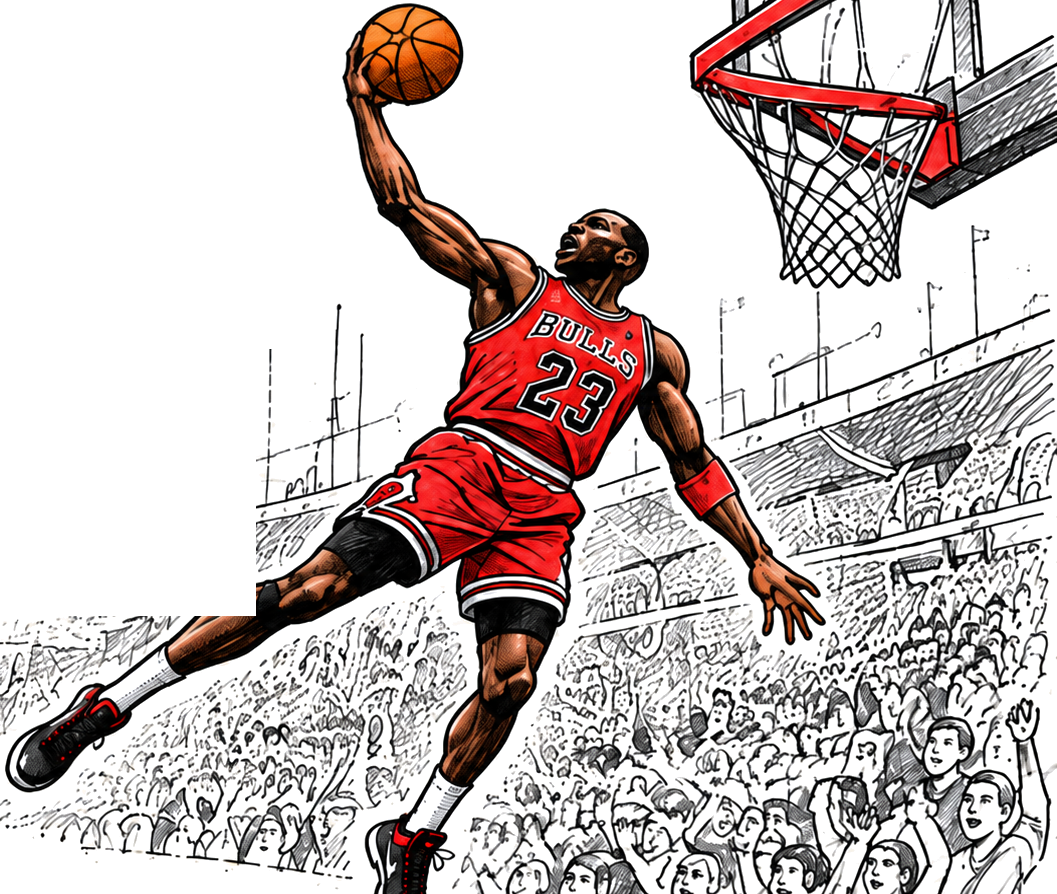
\includegraphics[width=\linewidth,height=6.3cm,keepaspectratio]{art_cover.png}
\end{column}
\end{columns}
\end{frame}

% 02 --- PREFACIO

\begin{frame}{Prefácio}
\begin{columns}[T,onlytextwidth]
\begin{column}{.60\textwidth}
\vspace{.22cm}
\large
Esta apresentação discute, de forma visual e didática, um problema simples de cinemática: \keyterm{quanto é necessário subir para permanecer um segundo no ar?}
\par\vspace{.37cm}
Por meio do basquete, exploraremos as leis do movimento, a interpretação física dos resultados e sua conexão com o desempenho de atletas.
\par\vspace{.43cm}
{\color{primary}\Large\itshape Boa física e bons saltos.}
\end{column}
\begin{column}{.38\textwidth}
\centering\vspace{-.17cm}
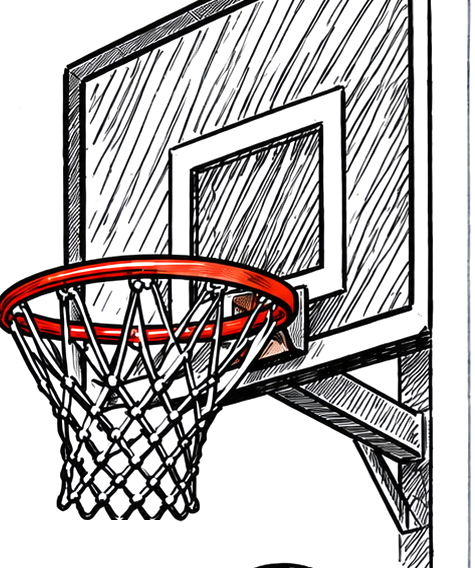
\includegraphics[height=4.0cm,width=\linewidth,keepaspectratio]{art_hoop.png}
\par\vspace{-.35cm}
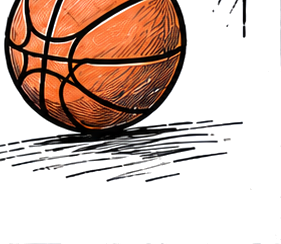
\includegraphics[height=1.65cm,keepaspectratio]{art_ball.png}
\end{column}
\end{columns}
\end{frame}

% 03 --- GLOSSARIO
\begin{frame}{Símbolos, termos e equações principais}
\vspace{.12cm}
\begin{columns}[T,onlytextwidth]
\begin{column}{.55\textwidth}
\renewcommand{\arraystretch}{1.21}
\begin{tabular}{@{}>{\color{primary}}l l@{}}
$y(t)$ & deslocamento vertical (m)\\
$v_0$ & velocidade inicial (m/s)\\
$g$ & aceleração da gravidade (m/s$^2$)\\
$t$ & tempo (s)\\
$T$ & tempo total de voo (s)\\
$h$ & altura máxima (m)\\
$t_{\max}$ & tempo até a altura máxima (s)
\end{tabular}
\end{column}
\begin{column}{.42\textwidth}
\begin{beamercolorbox}[sep=11pt,wd=\linewidth,rounded=true]{block body}
\small\keyterm{Valor adotado}\par\vspace{.10cm}
\centerline{$\displaystyle g\simeq 9{,}8\,\mathrm{m/s^2}$}
\vspace{.25cm}\keyterm{Unidades SI}\par
Comprimento: metro (m)\par
Tempo: segundo (s)\par
Velocidade: m/s\par
Aceleração: m/s$^2$
\end{beamercolorbox}
\end{column}
\end{columns}
\vspace{.07cm}
\sectionline{Equações principais (lançamento vertical)}
\begin{center}
\begin{tikzpicture}[every node/.style={draw=accent,fill=white,rounded corners=2pt,inner xsep=7pt,inner ysep=4pt},node distance=0.18cm]
\node (a) {$\displaystyle y(t)=v_0t-\frac{gt^2}{2}$};
\node[right=of a] (b) {$\displaystyle v_0=\frac{gT}{2}$};
\node[right=of b] (c) {$\displaystyle t_{\max}=\frac T2$};
\node[right=of c] (d) {$\displaystyle h=\frac{gT^2}{8}$};
\end{tikzpicture}
\end{center}
\end{frame}

% 04 --- ROTEIRO
\begin{frame}{Roteiro da apresentação}
\vspace{.22cm}
\begin{columns}[T,onlytextwidth]
\begin{column}{.49\textwidth}
\renewcommand{\arraystretch}{1.75}
\begin{tabular}{@{}>{\color{primary}\bfseries}r@{\qquad}l@{}}
01 & Pergunta-problema\\
02 & Modelo físico\\
03 & Equação do movimento\\
04 & Tempo total de voo\\
05 & Simetria do movimento\\
06 & Ponto mais alto
\end{tabular}
\end{column}
\begin{column}{.49\textwidth}
\renewcommand{\arraystretch}{1.75}
\begin{tabular}{@{}>{\color{primary}\bfseries}r@{\qquad}l@{}}
07 & Fórmula geral\\
08 & Caso de um segundo\\
09 & Como a altura cresce\\
10 & Maiores saltos verticais\\
11 & Michael Jordan e o \emph{hang time}\\
12 & Bibliografia
\end{tabular}
\end{column}
\end{columns}
\vspace{.56cm}
\begin{center}
{\color{accent}\large\bfseries Do problema à realidade: uma jornada em 12 passos.}
\end{center}
\end{frame}

% 05 --- RESUMO

\begin{frame}{Resumo: o que encontramos?}
\begin{columns}[T,onlytextwidth]
\begin{column}{.34\textwidth}
\centering\vspace{.03cm}
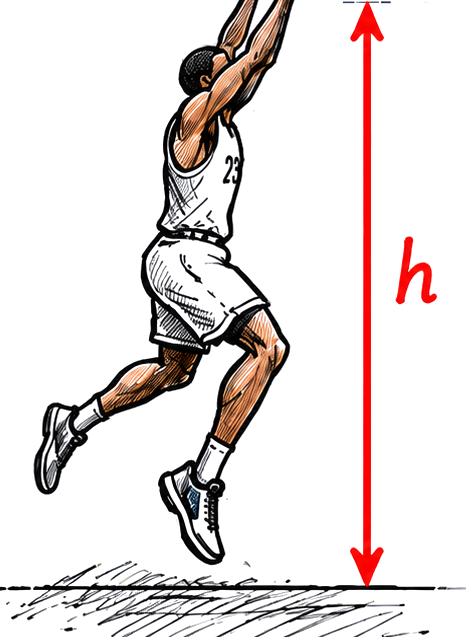
\includegraphics[width=\linewidth,height=5.9cm,keepaspectratio]{art_summary.png}
\end{column}
\begin{column}{.63\textwidth}
\large
O modelo de lançamento vertical fornece
\[\displaystyle T=\frac{2v_0}{g},\qquad h=\frac{gT^2}{8},\qquad t_{\max}=\frac T2.\]
\vspace{.04cm}
Para \alertterm{$T=1\,\mathrm{s}$}:
\begin{center}\eqcard{h\simeq1{,}23\,\mathrm{m}\qquad v_0\simeq4{,}9\,\mathrm{m/s}}\end{center}
\begin{itemize}\setlength{\itemsep}{.11cm}
\item A altura cresce com o quadrado do tempo: $h\propto T^2$.
\item Um segundo de voo exige um salto vertical excepcional no modelo ideal.
\end{itemize}
\end{column}
\end{columns}
\end{frame}

% 06 --- PROBLEMA

\begin{frame}{1. Qual é o problema?}
\vspace{.15cm}
\begin{center}
{\fontsize{22}{27}\selectfont Quanto é necessário saltar para permanecer\\[.10cm] \alertterm{1 segundo no ar}?}
\end{center}
\vspace{.14cm}
\begin{center}
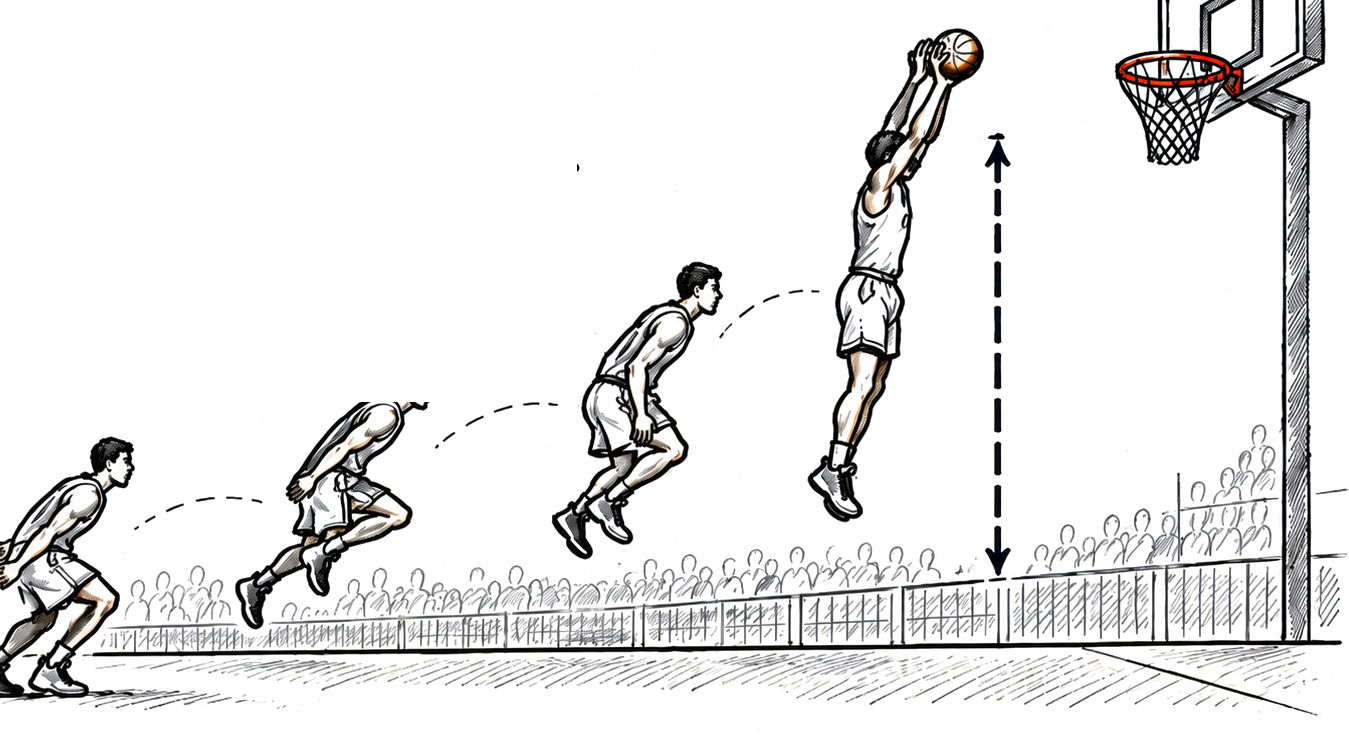
\includegraphics[width=12.6cm,height=3.86cm,keepaspectratio]{art_sequence.png}
\end{center}
\end{frame}

% 07 --- MODELO

\begin{frame}{2. Modelo físico}
\begin{columns}[T,onlytextwidth]
\begin{column}{.54\textwidth}
\vspace{.43cm}
\large
\begin{itemize}\setlength{\itemsep}{.39cm}
\item Salto vertical ideal.
\item Resistência do ar desprezada.
\item Decolagem e aterrissagem na mesma altura.
\item Somente a gravidade atua durante o voo.
\end{itemize}
\end{column}
\begin{column}{.44\textwidth}
\centering
\begin{tikzpicture}[x=1cm,y=1cm]
\node[anchor=south west,inner sep=0] at (0.2,0.05) {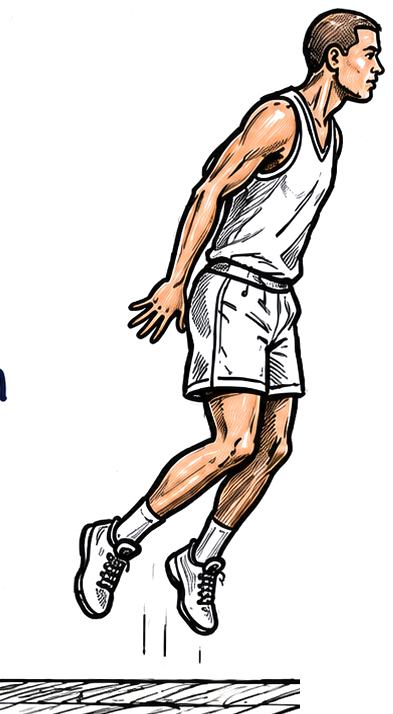
\includegraphics[height=5.45cm]{art_model.png}};
\draw[primary,line width=1.6pt,-{Stealth[length=2.9mm]}] (3.9,2.7)--(3.9,5.10);
\node[primary,right] at (3.95,4.73) {$v_0$};
\draw[accent,line width=1.6pt,-{Stealth[length=2.9mm]}] (4.6,4.54)--(4.6,2.44);
\node[accent,right] at (4.68,3.25) {$g$};
\node[accent,align=center,font=\scriptsize] at (3.86,1.40) {$g\simeq 9{,}8\,\mathrm{m/s^2}$};
\end{tikzpicture}
\end{column}
\end{columns}
\end{frame}

% 08 --- EQUACAO
\begin{frame}{3. Equação do movimento}
\vspace{.13cm}
\begin{columns}[T,onlytextwidth]
\begin{column}{.54\textwidth}
\large Cinemática no eixo vertical:
\vspace{.24cm}
\begin{center}\eqcard{y(t)=v_0t-\frac{1}{2}gt^2}\end{center}
\vspace{.35cm}
\begin{tabular}{@{}>{\color{primary}}ll@{}}
$y(t)$: & deslocamento vertical\\[.12cm]
$v_0$: & velocidade inicial\\[.12cm]
$g$: & aceleração da gravidade
\end{tabular}
\end{column}
\begin{column}{.44\textwidth}
\centering
\begin{tikzpicture}
\begin{axis}[
 width=6.3cm,height=5.2cm,
 xmin=0,xmax=1.13,ymin=0,ymax=1.45,
 axis lines=left,axis line style={primary,thick,-{Stealth}},
 xlabel={$t$},ylabel={$y$},
 xtick=\empty,ytick=\empty,
 enlargelimits=false,
 every axis x label/.style={at={(axis description cs:1.03,-.04)},anchor=north},
 every axis y label/.style={at={(axis description cs:-.04,1.03)},anchor=south},
 clip=false]
\addplot[primary,very thick,domain=0:1,samples=80] {4.9*x-4.9*x*x};
\addplot[accent,mark=*,mark size=2.6pt,only marks] coordinates {(.5,1.225)};
\draw[muted,dashed] (axis cs:.5,0)--(axis cs:.5,1.225);
\end{axis}
\end{tikzpicture}
\end{column}
\end{columns}
\end{frame}

% 09 --- TEMPO

\begin{frame}{4. Tempo total de voo}
\begin{columns}[T,onlytextwidth]
\begin{column}{.60\textwidth}
\large O tempo total de voo é $T$. Como a decolagem e a aterrissagem ocorrem na mesma altura,
\[y(T)=0.\]
Substituindo a equação do movimento,
\[0=v_0T-\frac12 gT^2.\]
Para a solução não trivial $T>0$, obtemos
\vspace{-.16cm}\begin{center}\eqcard{v_0=\frac{gT}{2}}\end{center}
\end{column}
\begin{column}{.38\textwidth}
\centering\vspace{-.12cm}
\begin{tikzpicture}[x=1cm,y=1cm]
\node[anchor=south west,inner sep=0] at (0,0.0) {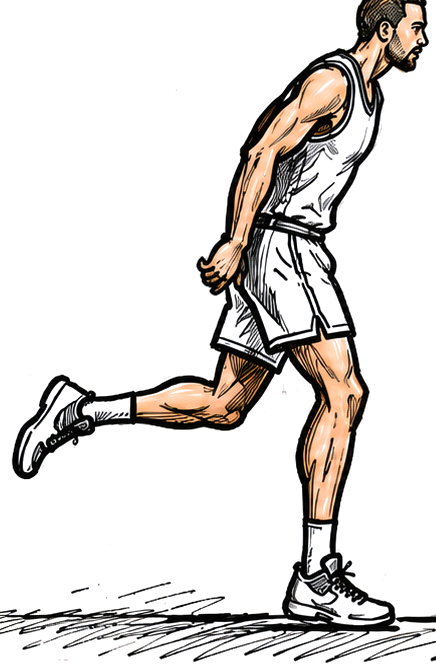
\includegraphics[height=5.38cm]{art_flight.png}};
\draw[accent,line width=1.7pt,{Stealth}-{Stealth}] (3.6,.16)--(3.6,4.75);
\node[accent,right] at (3.66,2.4) {$T$};
\end{tikzpicture}
\end{column}
\end{columns}
\end{frame}

% 10 --- SIMETRIA
\begin{frame}{5. Simetria do movimento}
\vspace{.04cm}
\begin{columns}[T,onlytextwidth]
\begin{column}{.52\textwidth}
\large
\begin{itemize}\setlength{\itemsep}{.19cm}
\item O movimento é simétrico em relação ao instante de altura máxima.
\item O tempo de subida é igual ao tempo de descida.
\end{itemize}
\end{column}
\begin{column}{.45\textwidth}
\centering\vspace{.15cm}\eqcard{t_{\max}=\frac T2}
\end{column}
\end{columns}
\vspace{.16cm}
\begin{center}
\begin{tikzpicture}[x=1cm,y=1cm]
\draw[primary,thick,-{Stealth}] (0,.4)--(12.3,.4) node[right] {$t$};
\draw[primary,line width=1.6pt,domain=0:10.3,samples=95] plot(\x,{.4+1.0*\x-.0971*\x*\x});
\draw[accent,dashed,thick] (5.15,.4)--(5.15,2.98);
\draw[accent,fill=accent] (5.15,2.98) circle (.07);
\draw[primary,fill=primary] (0,.4) circle (.06);
\draw[primary,fill=primary] (10.3,.4) circle (.06);
\node[primary,align=center] at (2.75,1.31) {Subida\\$T/2$};
\node[primary,align=center] at (7.55,1.31) {Descida\\$T/2$};
\draw[accent,line width=1pt,{Stealth}-{Stealth}] (0,-.12)--(10.3,-.12);
\node[accent,below] at (5.15,-.12) {$T$};
\end{tikzpicture}
\end{center}
\end{frame}

% 11 --- PONTO ALTO

\begin{frame}{6. Ponto mais alto}
\begin{columns}[T,onlytextwidth]
\begin{column}{.53\textwidth}
\vspace{.30cm}
\large No ponto mais alto da trajetória:
\begin{itemize}\setlength{\itemsep}{.24cm}
\item A velocidade instantânea é nula: $v=0$.
\item A altura máxima é obtida de $v^2=v_0^2-2gy$.
\end{itemize}
\vspace{.30cm}
\begin{center}\eqcard{h=\frac{v_0^2}{2g}}\end{center}
\end{column}
\begin{column}{.44\textwidth}
\centering
\begin{tikzpicture}[x=1cm,y=1cm]
\draw[ink,thick] (-.1,.4)--(4.4,.4);
\draw[ink,dashed,line width=1.1pt,domain=.35:4.1,samples=50] plot(\x,{.4+2.35*(1-((\x-2.225)/1.875)^2)});
\draw[accent,fill=accent] (2.225,2.75) circle (.085);
\node[accent,above] at (2.225,2.82) {$v=0$};
\draw[accent,line width=1.5pt,{Stealth}-{Stealth}] (2.225,.42)--(2.225,2.65);
\node[accent,right] at (2.28,1.45) {$h$};
\node[anchor=south west,inner sep=0] at (-.25,.45) {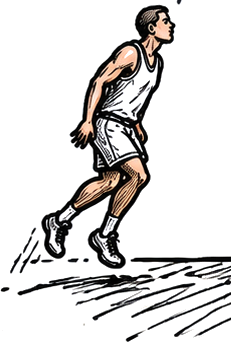
\includegraphics[height=2.35cm]{art_apex.png}};
\end{tikzpicture}
\end{column}
\end{columns}
\end{frame}

% 12 --- FORMULA GERAL
\begin{frame}{7. Fórmula geral}
\begin{columns}[T,onlytextwidth]
\begin{column}{.72\textwidth}
\vspace{.1cm}
\large Usando $v_0=gT/2$ na expressão da altura máxima,
\begin{align*}
 h&=\frac{v_0^2}{2g}
   =\frac{(gT/2)^2}{2g}\\[-.04cm]
  &=\frac{g^2T^2}{8g}.
\end{align*}
\vspace{-.35cm}
\begin{center}\eqcard{h(T)=\frac{gT^2}{8}}\end{center}
\vspace{-.28cm}
\normalsize Portanto, a altura necessária para permanecer $T$ segundos no ar cresce com o \keyterm{quadrado do tempo}, isto é, $h\propto T^2$.
\end{column}
\begin{column}{.27\textwidth}
\centering\vspace{-.05cm}
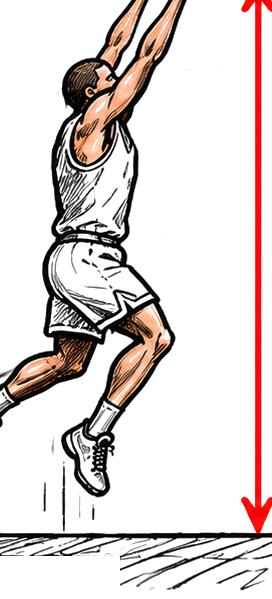
\includegraphics[width=\linewidth,height=5.75cm,keepaspectratio]{art_general.png}
\end{column}
\end{columns}
\end{frame}

% 13 --- UM SEGUNDO

\begin{frame}{8. Um segundo no ar}
\begin{columns}[T,onlytextwidth]
\begin{column}{.64\textwidth}
\vspace{.18cm}
{\Large Para \alertterm{$T=1\,\mathrm{s}$}:}
\vspace{.22cm}
\[h=\frac{gT^2}{8}
  =\frac{9{,}8\cdot(1)^2}{8}\,\mathrm{m}.\]
\begin{center}\eqcard{h\simeq 1{,}23\,\mathrm{m}}\end{center}
\vspace{.26cm}
\large É necessário elevar o centro de massa em cerca de $1{,}23$ metro entre a decolagem e o ponto mais alto.
\end{column}
\begin{column}{.34\textwidth}
\centering\vspace{-.12cm}
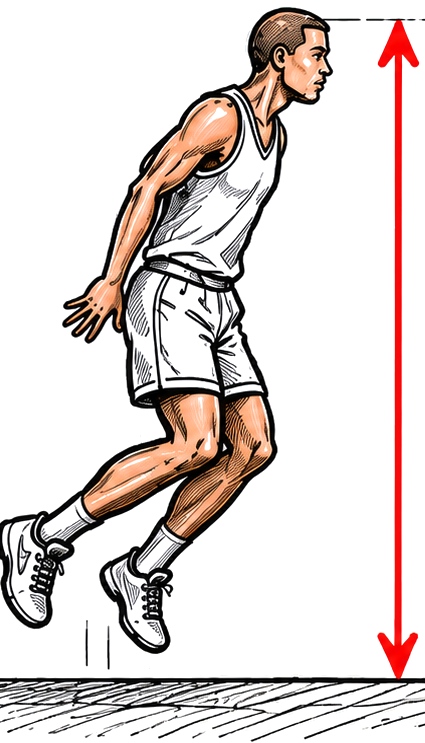
\includegraphics[width=\linewidth,height=5.92cm,keepaspectratio]{art_one_second.png}
\end{column}
\end{columns}
\end{frame}

% 14 --- CRESCIMENTO
\begin{frame}{9. Como a altura cresce}
\begin{columns}[T,onlytextwidth]
\begin{column}{.24\textwidth}
\vspace{.38cm}\begin{center}\eqcard{h\propto T^2}\end{center}
\vspace{.47cm}
\large Dobrar o tempo no ar exige \alertterm{quadruplicar} a altura do salto.
\end{column}
\begin{column}{.49\textwidth}
\centering
\begin{tikzpicture}
\begin{axis}[
  width=7.1cm,height=5.25cm,
  xmin=0,xmax=2.15,ymin=0,ymax=5.35,
  xlabel={$T\;(\mathrm{s})$}, ylabel={$h\;(\mathrm{m})$},
  axis lines=left,axis line style={primary,thick,-{Stealth}},
  tick label style={font=\scriptsize},
  xlabel style={font=\small},ylabel style={font=\small},
  xtick={0,.5,1,1.5,2},ytick={0,1,2,3,4,5},
  grid=both, grid style={gridgray!55,thin},
  clip=false]
\addplot[primary,very thick,domain=0:2.03,samples=90] {9.8*x*x/8};
\addplot[accent,only marks,mark=*,mark size=2.6pt] coordinates {(.5,.30625) (1,1.225) (1.5,2.75625) (2,4.9)};
\end{axis}
\end{tikzpicture}
\end{column}
\begin{column}{.25\textwidth}
\vspace{.86cm}
\renewcommand{\arraystretch}{1.32}
\begin{tabular}{@{}>{\color{primary}}r r@{}}\toprule
$T$ (s)&$h$ (m)\\\midrule
$0{,}5$&$0{,}31$\\
$1{,}0$&$1{,}23$\\
$1{,}5$&$2{,}76$\\
$2{,}0$&$4{,}90$\\\bottomrule
\end{tabular}
\end{column}
\end{columns}
\end{frame}

% 15 --- REGISTROS

\begin{frame}{10. Maiores saltos verticais}
\vspace{.01cm}
\large Valores apresentados no material de origem:
\vspace{.16cm}
\begin{columns}[T,onlytextwidth]
\begin{column}{.17\textwidth}
\centering\vspace{.5cm}
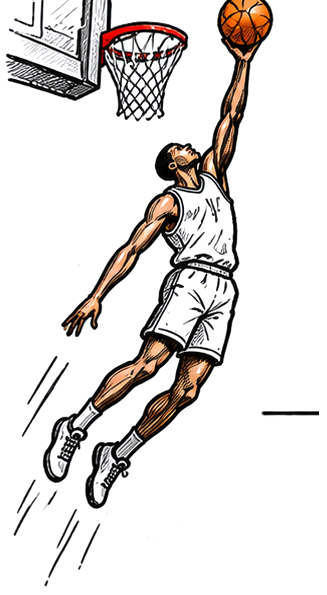
\includegraphics[width=\linewidth,height=4.8cm,keepaspectratio]{art_records.png}
\end{column}
\begin{column}{.81\textwidth}
\begin{tikzpicture}
\begin{axis}[
 width=10.8cm,height=4.91cm,
 xmin=.40,xmax=5.6,ymin=0,ymax=1.62,
 axis lines=left,axis line style={ink,thick},
 ytick={0,.4,.8,1.2,1.6},yticklabel style={font=\scriptsize},
 xtick={1,2,3,4,5},
 xticklabels={{Darius Clark\\(2022)},{Darius Clark\\(2025)},{Dylan McCarthy\\(2026)},{Ethan Pimstone\\(2026)},{Darius Clark\\(2026)}},
 x tick label style={font=\tiny,align=center},
 ylabel={Altura (m)},ylabel style={font=\small},
 grid=major, ymajorgrids=true,xmajorgrids=false,grid style={gridgray!45},
 enlarge x limits=false,clip=false]
\addplot[ybar,bar width=.43cm,draw=accent,fill=basket!72,mark=none] coordinates {(1,1.27) (2,1.30) (3,1.32) (4,1.35) (5,1.35)};
\node[above,font=\tiny\bfseries,text=accent] at (axis cs:1,1.295) {1,27\,m};
\node[above,font=\tiny\bfseries,text=accent] at (axis cs:2,1.325) {1,30\,m};
\node[above,font=\tiny\bfseries,text=accent] at (axis cs:3,1.345) {1,32\,m};
\node[above,font=\tiny\bfseries,text=accent] at (axis cs:4,1.375) {1,35\,m};
\node[above,font=\tiny\bfseries,text=accent] at (axis cs:5,1.375) {1,35\,m};
\end{axis}
\end{tikzpicture}
\end{column}
\end{columns}
\vspace{-.07cm}
{\color{muted}\scriptsize Nota: os nomes, anos e valores foram transcritos do PDF fornecido; os respectivos registros e protocolos de medição não foram verificados independentemente.}
\end{frame}

% 16 --- JORDAN

\begin{frame}{11. Michael Jordan e o \emph{hang time}}
\begin{columns}[T,onlytextwidth]
\begin{column}{.42\textwidth}
\centering\vspace{.09cm}
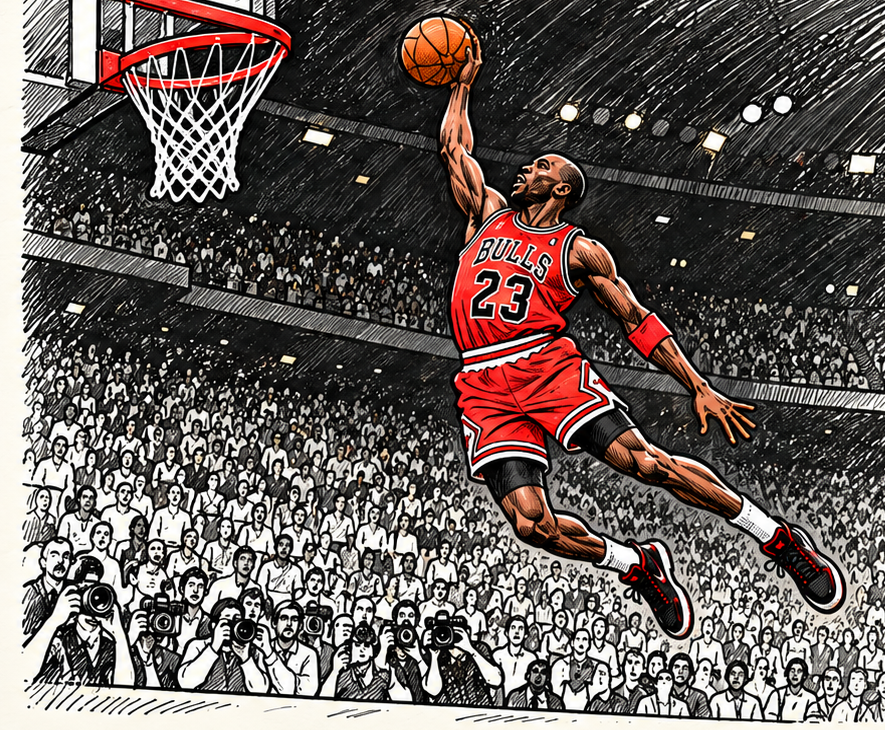
\includegraphics[width=\linewidth,height=5.45cm,keepaspectratio]{art_jordan.png}
\end{column}
\begin{column}{.55\textwidth}
\vspace{.14cm}
\large
\begin{itemize}\setlength{\itemsep}{.12cm}
\item Um dos saltos mais conhecidos do basquete ocorreu no \emph{Slam Dunk Contest} de 1988.
\item A vertical de 48 polegadas ($\approx1{,}22\,\mathrm{m}$), frequentemente mencionada, requer cautela metodológica.
\item O material didático original apresenta uma estimativa de tempo de voo da ordem de \alertterm{$0{,}92\,\mathrm{s}$}.
\end{itemize}
\vspace{.06cm}
{\color{muted}\footnotesize Uma distância vertical e um tempo de voo não são intercambiáveis sem explicitar os respectivos procedimentos de medição.}
\end{column}
\end{columns}
\end{frame}

% 17 --- BIBLIOGRAFIA

\begin{frame}{12. Bibliografia e referências}
\begin{columns}[T,onlytextwidth]
\begin{column}{.28\textwidth}
\centering\vspace{.72cm}

\includegraphics[width=\linewidth,height=5.06cm,keepaspectratio]{art_books.png}
\end{column}
\begin{column}{.70\textwidth}
\vspace{-.13cm}
\sectionline{Livros de física}
\begin{itemize}\setlength{\itemsep}{.06cm}
\item Serway e Jewett, \emph{Física para Cientistas e Engenheiros}.
\item Halliday, Resnick e Walker, \emph{Fundamentos de Física}.
\item Tipler e Mosca, \emph{Física para Cientistas e Engenheiros}.
\item Nussenzveig, \emph{Curso de Física Básica}.
\end{itemize}
\vspace{.05cm}
\sectionline{Referências adicionais indicadas no material original}
\begin{itemize}\setlength{\itemsep}{.04cm}
\item Guinness World Records.
\item Dunk Camp.
\item NBA -- \emph{Slam Dunk Contest} de 1988.
\item TED-Ed -- \emph{Hang time} de Michael Jordan.
\end{itemize}
\vspace{-.12cm}
{\color{muted}\scriptsize Referências preservadas como no documento-fonte; edições e endereços eletrônicos não especificados.}
\end{column}
\end{columns}
\end{frame}

% 18 --- AUTOR

\begin{frame}{Sobre o autor}
\vspace{.12cm}
\begin{columns}[T,onlytextwidth]
\begin{column}{.53\textwidth}
{\Large\bfseries\color{primary} Osvaldo L. Santos-Pereira}\par\vspace{.15cm}
{\large Instituto de Física\\ Universidade Federal do Rio de Janeiro (UFRJ)}
\vspace{.42cm}
\large Físico interessado no ensino e na divulgação científica, bem como na utilização de ferramentas de inteligência artificial para a criação de recursos didáticos.
\end{column}
\begin{column}{.43\textwidth}
\sectionline{Áreas de interesse}
\begin{itemize}\setlength{\itemsep}{.07cm}
\item Física teórica
\item Ensino de física
\item Divulgação científica
\item Comunicação e visualização
\item Inteligência artificial
\end{itemize}
\vspace{.25cm}
\sectionline{Perfis acadêmicos e profissionais}
{\small ORCID \enspace$\cdot$\enspace Google Scholar \enspace$\cdot$\enspace Lattes\\[.07cm]
GitHub \enspace$\cdot$\enspace LinkedIn}
\end{column}
\end{columns}
\begin{tikzpicture}[remember picture,overlay]
\node[anchor=north east,inner sep=0] at ([xshift=-.82cm,yshift=-.93cm]current page.north east) {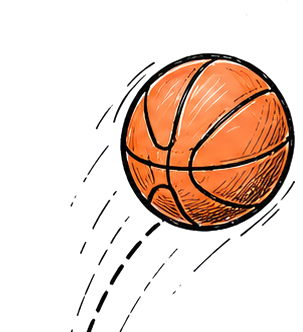
\includegraphics[width=1.28cm]{art_basketball.png}};
\end{tikzpicture}
\vfill
\begin{center}{\color{accent}\large\itshape Boas ideias também podem nascer de boas perguntas.}\end{center}
\end{frame}

\end{document}
